
\chapter{Stacking Methodology}
Given the signal from a single filament is well below the level of noise in a given $y$ map, in order to effectively detect the signal for the filaments, we need to add many individual sources together. Because the noise, and the signal in the CMB is presumed to be gaussian, the expectation is that correlated signals would add, and uncorrelated signals would be driven to zero. This means that by adding together thousands of signals lower than the signal-to-noise ratio of a given $y$ map, it should show the filaments as a correlated signal, along with their corresponding galactic halos.

Initially outlined in \cite{2016MNRAS.457.2391C}, the stacking algorithm involves creating a list of galaxy pairs, which we would expect to see a filament between, and then using those pairs, forming a normalised two-dimensional image, with the galaxies of the pair being placed on two points in the image, and stacking them until the signal to noise is sufficient to be measurable.

The intial problem faced involves generating the galaxy pairs from the Dark Energy Survey redMaGiC Catalogue. The Year 1 Catalogue consists of 0.65 million red-sequence galaxies in the redshift range $0.15 < z < 0.9 $. The algorithm used by the Dark Energy Survey to select these red-sequence galaxies provides redshift estimates of very high quality and very low bias ($\lesssim 0.5$ percent). They also have very low scatter, and a very low rate of catastrophic outliers. The algorithm yields superior photo-z performance than the colour-cut methodology used to define the Sloan Digital Sky Survey CMASS catalogue \citep{2016MNRAS.461.1431R}. 

The DES catalogue has a larger footprint than the SPTpol viewing footprint, so we first have to exclude any galaxies that lie outside of the SPTpol area. The SPTpol observing area consists of a 500 square degree patch of sky, extending from an Right Acension (RA) of 22h to 2h, and a Declination (Dec) of -52 degrees to -67 degrees. Excluding any galaxies outside this region yields approximately 100000 galaxies, less than a sixth of the original catalogue. 

\begin{figure}[h!]
\centering 
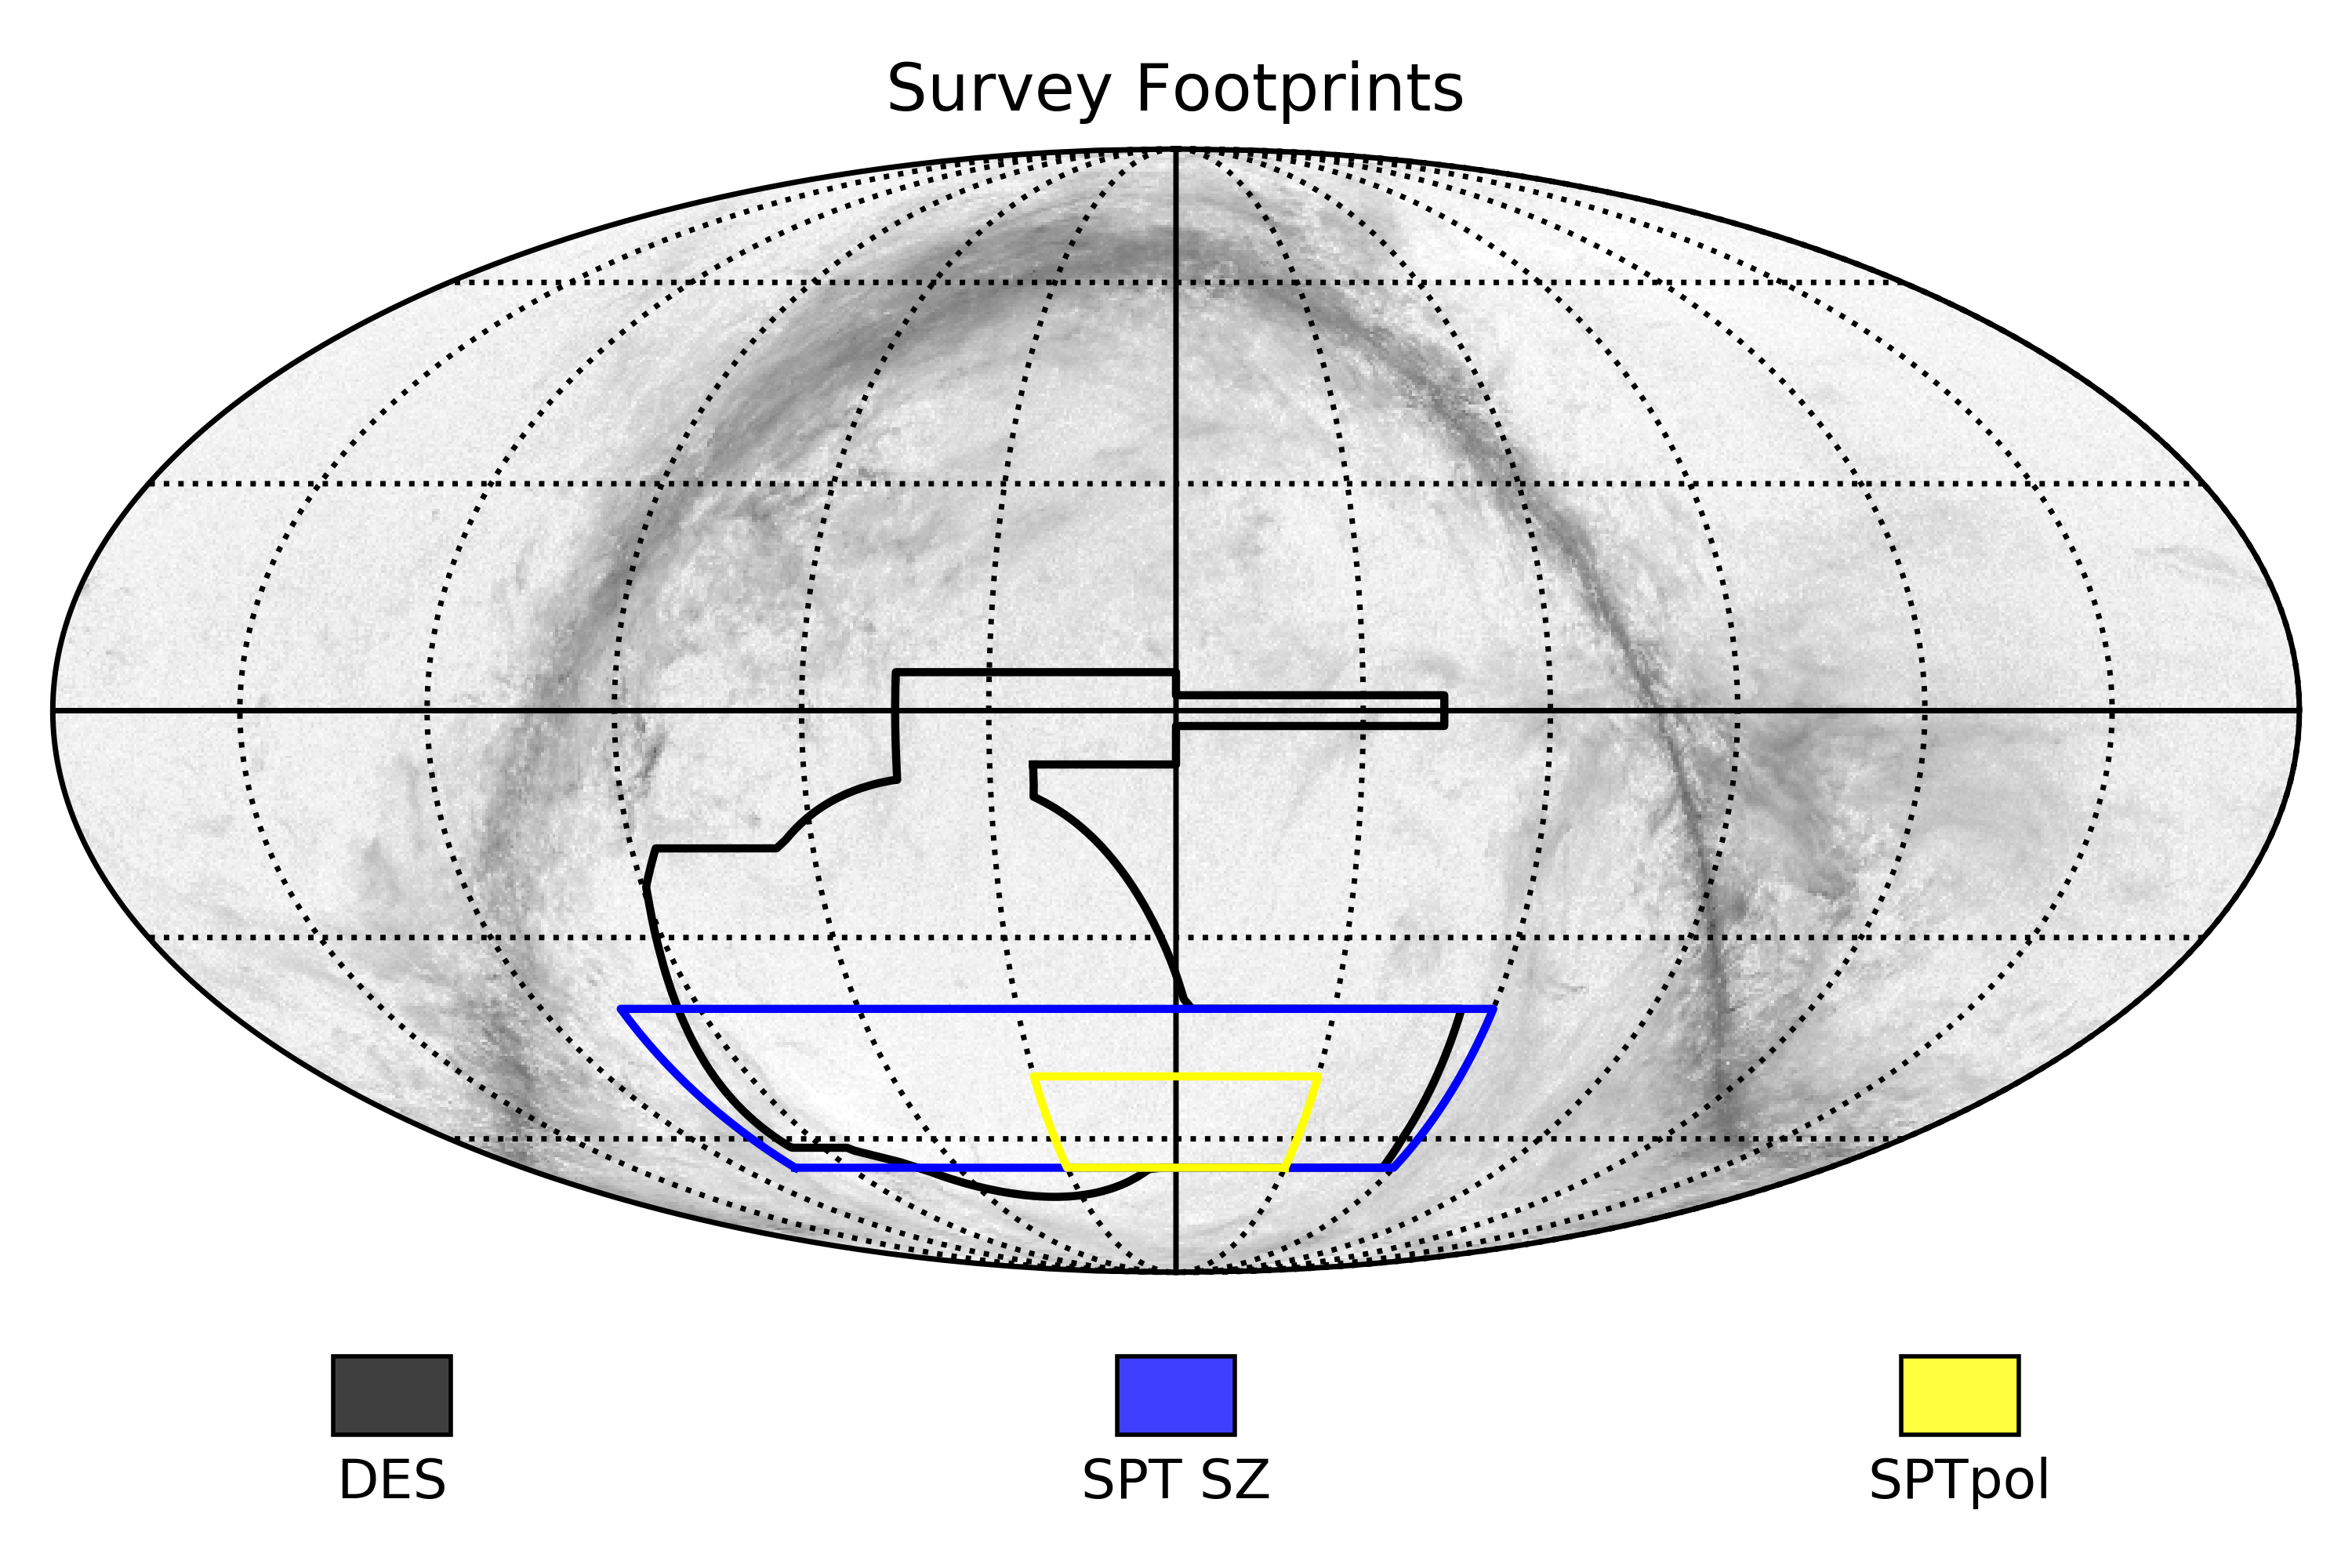
\includegraphics[scale=0.7]{/home/mitchell/Documents/masters/masters/thesis/Ver_2/figures/Survey_Outlines.png}
\caption{Outlines of SPTpol, SPT-SZ, and DES surveys}
\label{fig:surveys}
\end{figure}



Pairs were generated by making use of kD-trees. A generalisation of a binary tree, the kD tree is one where every leaf node is representative of a $k$ dimensional point. Each non-leaf node is one that 'splits' the space into two parts, whereby points to the left of this hyperplane are represented by the left sub-tree, and to the right are represented by the right sub-tree. When we apply this to our galaxy catalogue, we first locate them in 3 dimensional space, by converting their RA, Dec, and redshift into a comoving 3D coordinate. They are then placed in a kD tree, and any pair which has a radial comoving separation of less that $10 h^{-1} $ Mpc, and transverse comoving separation range of $6 - 14 h^{-1} $ Mpc is considered to have a filament \citep{2016MNRAS.457.2391C}.

From this, approximately 340,000 galaxy pairs were constructed with a mean angular separation of $\sim 31.6 $ arcmins, and a mean comoving separation of $11.9 h^{-1}$ Mpc. 
\begin{figure}[h!]
\centering
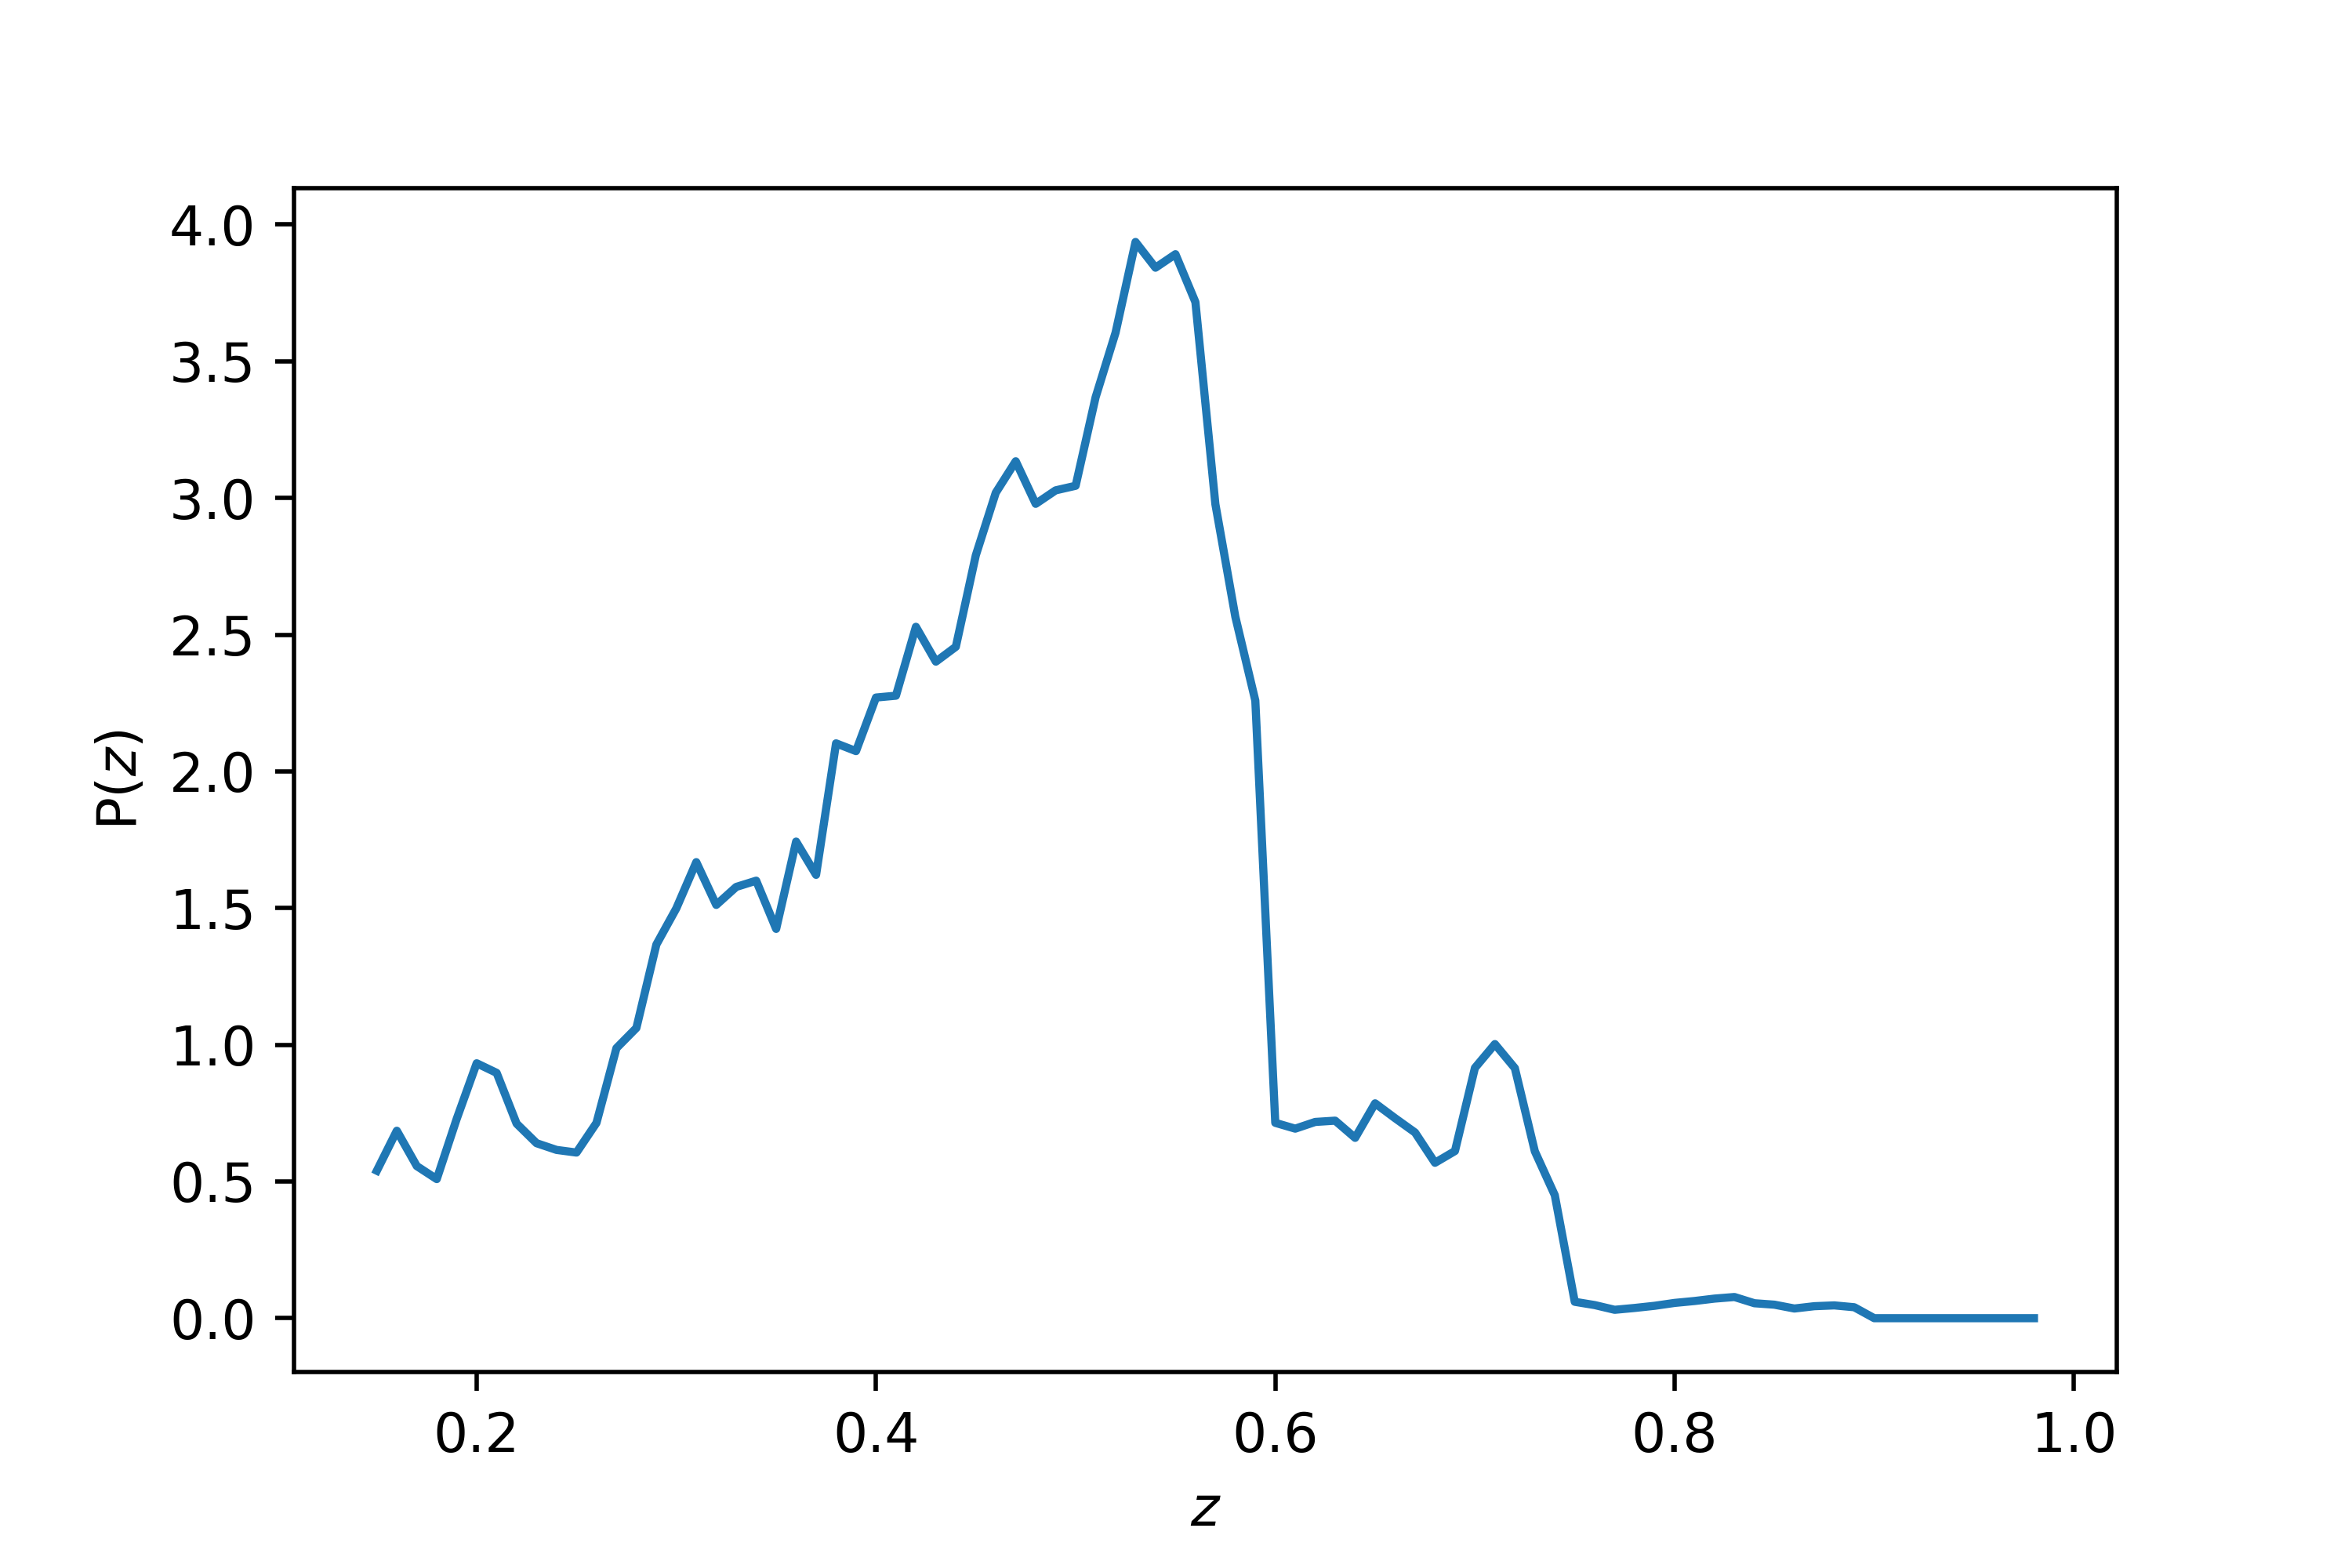
\includegraphics[scale=0.7]{/home/mitchell/Documents/masters/masters/thesis/Ver_2/figures/Redshift_Distribution.png}
\caption{Redshift Distribution of Galaxy Pairs}
\label{fig:pairs_dist}
\end{figure}

Figure \ref{fig:pairs_dist} shows the overall distribution of galaxy pairs as a function of redshift. It shows that the mean redshift for the pairs is $z=0.468$, with a minumum redshift of $z= 0.150$, and a maximum redshift of $z= 0.899$. There is a rather drastic drop in the galaxy population after redshift $z \sim 0.58$. This is due to there being fewer galaxies in the higher redshift bins in the DES Year 1 Catalgogue.  


Functionally, this means that the pair is located in the CMB, and a cutout of the CMB is taken around them, shown in Figure \ref{fig:first_cut}. We can see that this shows features we expect to see in the CMB, within characteristic ranges, and with a $y$-parameter measure given by the color bar. 

\begin{figure}[h!]
\centering 
\includegraphics[scale=0.8]{/home/mitchell/Documents/masters/masters/data/server/run_42/steps/1_firstcut.png}
\caption{Initial Slice of CMB}
\label{fig:first_cut}
\end{figure}

They are then rotated, so they are all aligned along the same axis. This is done by applying an affine transformation to the array of values, because we are seeking to preserve the functional position of all points, straight lines, and ratios in the array, as close to the original as possible. 

\begin{figure}[h!]
\centering 
\includegraphics[scale=0.8]{/home/mitchell/Documents/masters/masters/data/server/run_42/steps/1_rotated.png}
\caption{Rotated Cut-Out}
\label{fig:rotated}
\end{figure}

This subsequent image is then rescaled, so that each pair is located at the same point in the image.

\begin{figure}[h!]
\centering 
\includegraphics[scale=0.8]{/home/mitchell/Documents/masters/masters/data/server/run_42/steps/1_rescaled.png}
\caption{Rescaled Cut-Out}
\label{fig:rescaled}
\end{figure}

Now that the pair has been rescaled and rotated correctly, we slice around the centre of the array, given that the two galaxies in a given pair have been positioned on the same points. 
\begin{figure}[h!]
\centering 
\includegraphics[scale=0.8]{/home/mitchell/Documents/masters/masters/data/server/run_42/steps/1_secondcut.png}
\caption{Second Cut-Out}
\label{fig:second_cut}
\end{figure}

Now that the galaxy pair has been aligned, we calculate an average of the array, flipped along both the x and y axes.

\begin{figure}
\centering
\includegraphics[scale=1]{/home/mitchell/Documents/masters/masters/data/server/run_42/steps/1_average.png}
\caption{Average of Mirrored Arrays}
\label{fig:average_cut}
\end{figure}

We do this in an effort to force the halos to be spherically symmetric. 